\documentclass[]{report}

\usepackage{cite}
\usepackage{amsmath}
%\usepackage{algorithm}
\usepackage{pgfgantt}
\usepackage[noend]{algpseudocode}
\usepackage[]{algorithm2e}
\usepackage{graphicx}
\usepackage[
top    = 2.50cm,
bottom = 2.50cm,
left   = 2.75cm,
right  = 2.75cm]{geometry}
\usepackage{fancyhdr}
\pagestyle{fancy}
\lhead{COMP3003 - Project Proposal }
\rhead{Jonathan Foot - psyjpf}

\begin{document}

\begin{titlepage}
	\begin{center}
		\vspace*{1cm}
		\Huge
		\textbf{A Data-Driven Approach To Bus Timetable Optimisation Recommendations.}
		
		\LARGE
		\vspace{0.5cm}
		\textbf{Project Proposal}
		
		\vspace{1.5cm}
		
		\textbf{Jonathan Foot}
		
		psyjpf@nottingham.ac.uk
		
		
		\vspace{2.5cm}
		
		A project proposal for the degree of\\
		MSci Computer Science
		
		
		\vfill
		
		
\includegraphics[width=200px]{images/nottingham-logo.png}
	\end{center}
\end{titlepage}



\section*{Background and Motivation}
Bus transit systems remains the UK's leading public transportation method, with the average UK resident making 48 trips annually \cite{RN9}. Bus networks allow for a relatively low initial infrastructural investment, while offering great adaptability and environmental benefits; particularly with the popularity of hydrogen, electric and bio-gas buses increasing. Although, private transportation methods still remain the UK's preferred method of transport, with the average person taking 602 trips by car \cite{RN9}, over 12 times that of the number of bus trips. 

\vspace{0.5cm}
One of the leading deterrents for greater adoption of bus transportation is ``a belief that buses cannot be relied on to stick to their timetables''\cite{RN10}. Transport operators are responsible for the network route design, setting the frequencies, timetables and assigning vehicles and drivers to trips. When creating the timetable operators must consider both external factors, such as traffic, roadworks, severe weather, sporting events and internal factors, such as delays from previous trips affecting the subsequent trips and delays on passenger boarding and alighting \cite{RN11}.

\vspace{0.5cm}
The UK Senior Traffic Commissioner’s guidelines are for 95\% of buses to be “on-time”, which is defined as arriving between 1 minute early to 5 minutes late at a timing point\cite{RN14}. If bus operators repeatedly fail to adhere to this guideline, they can be fined up to £550 per vehicle \cite{RN14}. One way to ensure compliance is to add a significant amount of excess wait times at stops to recoup for any delays. But this will increase journey times and unneeded waiting can be considered “dead time” where the bus operator is not making any money. Creating a reliable timetable is therefore important to both the operators and customers alike.


\vspace{0.5cm}
98\% of buses in Great Britain are equipped with automatic vehicle location (AVL) devices\cite{RN12}, which is used to monitor the punctuality of buses to a high degree of accuracy. With some operators even storing the exact longitudinal and latitudinal position of every bus, up-to every 30 seconds. There is more data about buses than ever-before and with the United Kingdom Government legislating the Bus Service Act 2017\cite{RN13}, bus open data is becoming increasingly more accessible. It is my intentions that this open-data can be used to drive an optimisation algorithm to improve average on-time performance and instil greater customer confidence in bus timetables and using buses as a form of transport.


\vspace{0.5cm}
There is already a large amount of research in this area and bus timetable setting can be described as an NP-Hard problem \cite{RN15}. There are also many external factors to consider when creating a timetable, such as how does it connect with train times, school times, other bus routes and the number of available vehicles and drivers. It is therefore impractical to believe a single algorithm would be capable of generating a perfect new timetable but can instead be used to provide recommendations for bus operators to follow.


\section*{Aims and Objectives}


The end-user of the program is bus operators, I aim to create a program which will take in their historic timetables and bus times and then output newly optimised timetables; which should increase the buses average on-time performance. The program will try to find weeks where performance patterns were similar and suggest multiple different timetables for different parts of the years, to deal with demands and conditions changing throughout the year; for example, school summer holidays. 

\vspace{0.5cm}
 I have decided to use the Reading Buses Open Data API, due to it being an exemplary bus open data source, providing a year's worth of historic data. As well, as having previous development experience using it and local knowledge of the routes and destination, which might aid my understanding for any erroneous data received. 

\vspace{0.5cm}
The following lists my main objectives I intend to achieve:


\begin{enumerate}
	\item Interface with the Reading Buses Open Data API, request and download data required from the API.
%		\subitem a. Abstract the library, creating a modular design so that any other bus companies API feed could be used in future.
%	\item Ascertain the data quality and identify any areas where data is missing, incomplete or looks erroneous.
%	\item Remove or replace any data which is deemed as suspicious to minimise optimisation issues later on.
%		\subitem a. Decide upon a method for resolving erroneous data.
	\item Search through the data for weekly patterns and group them, to create multiple-timetables for the year; one for each group.
%		\subitem a. Allow the bus operator to specify maximum number of groups.
%		\subitem b. Allow the bus operator to refuse a suggestion and ask for another suggestion. Rank suggestions, based on group similarities confidence.
%		\subitem b. Allow the bus operator to input their own groupings and provide an estimated similarity rating for the weeks.
	\item Generate the performance metrics, such as average on-time performance of the old timetable for the last year.
		\begin{enumerate}
		\item Use these metrics, to compare and contrast against the new timetable later. 
	\end{enumerate}
	\item Take in the historic vehicle data and generate a new optimised timetable, to minute accuracy.
	\begin{enumerate}
		\item Explore multiple different methods for timetable optimisation.
		\item The new timetable will try to minimise unneeded idle/dead time at timing points.	
		\item The new timetable will not consider constraints on number of vehicles, or drivers available. 
		\item The new timetable will not consider how these changes might affect connections between other routes timetables.
		\item The new timetable must bear some resemblance to the original headway times and will be restricted to prevent an overzealous solution.  
		\item The new timetable cannot alter the bus services route design.
	\end{enumerate}
	\item Produce a simulation/scoring system which can take in the proposed timetable and output estimated performance levels, to allow for comparison with original timetable.
%		\subitem a. Explore involving estimating passenger flow rate throughout the day.
	\item Create a user friendly GUI, which can graphically highlight the differences between the two timetables, to easily distinguish where the improvements have been made.  

%	\item Graphically highlight the differences between the two timetables, for the Operator to easily distinguish the improvements made.
%	\item Allow for the produced timetable to be exported, preferably in TransXChange format. 
\end{enumerate}



\section*{Work Plan}
My work-plan focuses in the first semester on creating the library to interface with the data-source API and then finding weekly service schedule patterns. In the second semester, I will start to develop the optimisation algorithm, a method for estimating a timetable's performance and an end-user friendly graphical user interface. 

\vspace{0.5cm}
Any testing, such as unit tests and integration testing has been included inside of the development times allocated. 

\vspace{0.5cm}
The work plan is only an estimation, the timeline will be re-evaluated at the start of the second semester, to add in additional work, or reschedule remaining work where needed.  

\graphicspath{ {images/} }
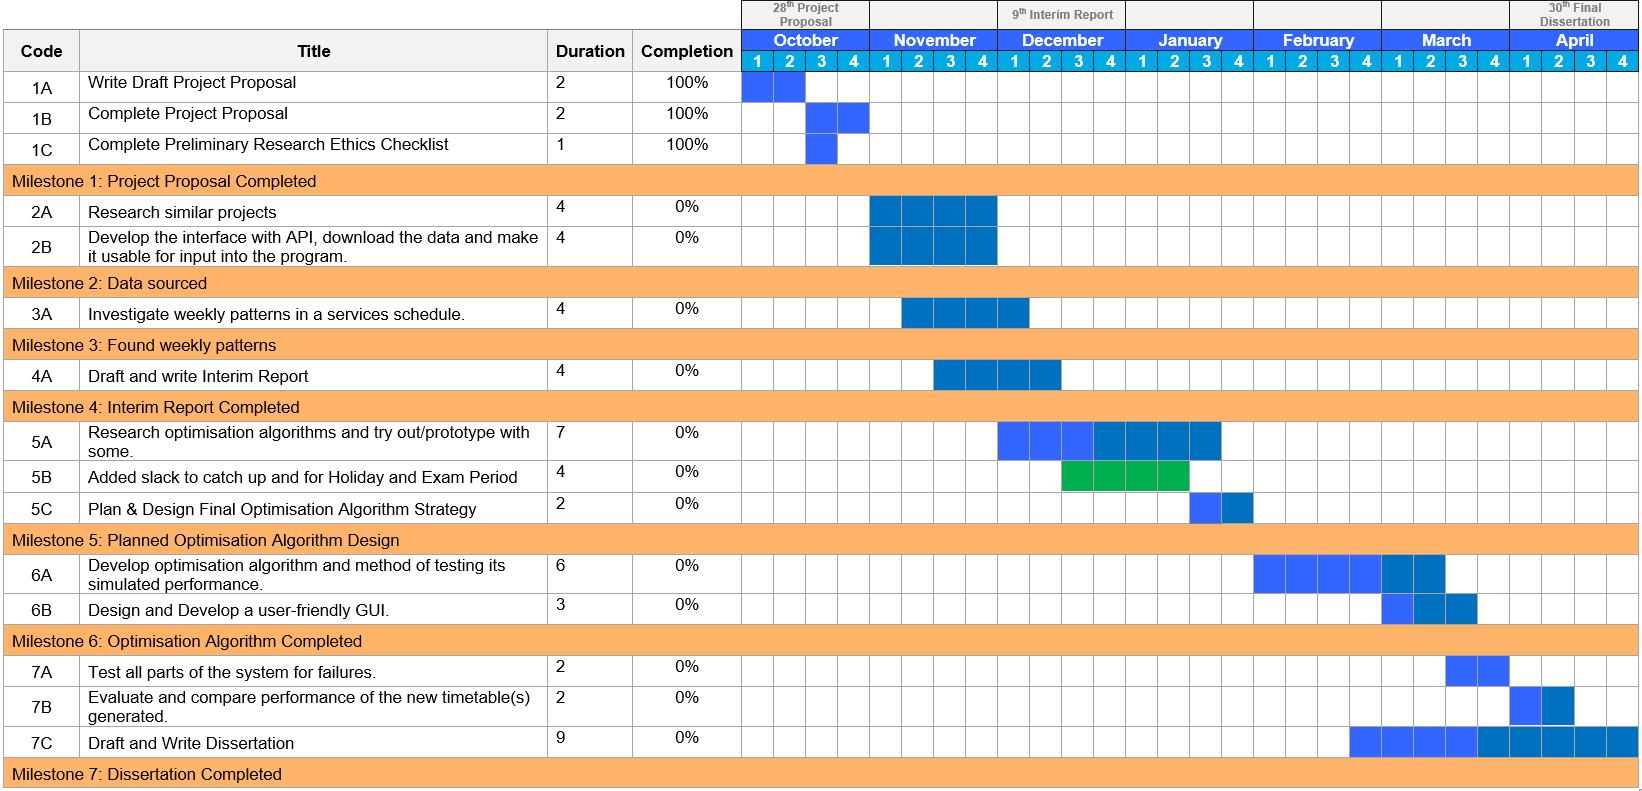
\includegraphics[width=\columnwidth]{ganntChartV2}

\section*{COVID-19 Considerations and Mitigations}
The historic bus data is retained for one year, after which it is removed from the API source. This means the majority of available data will be affected by COVID-19, which could result in usual or anomalous data. Particularly, where the official expected timetables were not updated with any temporary COVID-19 reduced timetable. Wherever possible, I shall aim to detect and remove anomalous data entries I suspect are a result of COVID-19. 

\vspace{0.5cm}
It is possible I may become ill during the year and this may affect my ability to work. If so the work-plan will have to be adjusted to reflect for any lost time. 
  
\vspace{0.5cm}
Going forwards, the project can be worked on remotely and I do not envisage any further issues, other than the continued aforementioned data quality issue.    

\section*{Conflicts of Interest}
I have previously been employed by Reading Buses as a freelance software-developer, the main data source provider for this project, but do not believe this shall have any effect on the overall project.

\vspace{0.5cm}
There are no other known conflicts of interest.

\bibliography{bibliography}
\bibliographystyle{plain}


\end{document}          
